\documentclass[a4paper,11pt]{article}

\usepackage[portuguese]{babel}
\usepackage[utf8]{inputenc}
\usepackage{amsmath}
\usepackage{graphicx}
\usepackage{hyperref}
\usepackage{float}
\usepackage{subfig}
\usepackage{fixltx2e}
\usepackage[bottom]{footmisc}
\usepackage{listings}
\usepackage{color} 
\usepackage[usenames,dvipsnames]{xcolor}
\usepackage[colorinlistoftodos]{todonotes}
\usepackage[font=footnotesize]{caption}

\usepackage[hypcap]{caption}
\usepackage[top=2.5cm, bottom=2.5cm, left=2.5cm, right=2.5cm]{geometry}
\usepackage{enumerate}

\numberwithin{equation}{section}
\addto\captionsportuguese{\renewcommand{\contentsname}{Índice}}

\linespread{1.3}
\usepackage{indentfirst}

\begin{document}
\begin{titlepage}
\begin{center}
	
\hfill \break
\hfill \break


\includegraphics[width=0.3\textwidth]{img/logo}~\\[1cm] 

\textsc{\LARGE Instituto Superior Técnico}\\[0.25cm]
\textsc{\Large Mestrado Integrado em Engenharia Electrotécnica e de Computadores}\\[1.8cm]
\textsc{\huge Electrónica de Potência}\\[0.25cm]

\vspace{6mm}

{\huge \bfseries Circuito de Disparo de um Tiristor \linebreak \& \linebreak Circuito com Carga Ressonante \linebreak Comutação pela Carga  \\[1cm]}

\begin{tabular}{ l l }
	João Bernardo Sequeira de Sá & \hspace{2mm} n.º 68254 \\
	Maria Margarida Dias dos Reis & \hspace{2mm} n.º 73099 \\
	Rafael Augusto Maleno Charrama Gonçalves & \hspace{2mm} n.º 73786 \\
	Nuno Miguel Rodrigues Machado & \hspace{2mm} n.º 74236
\end{tabular}

\vspace{7mm}

Grupo n.º TAL de segunda-feira das 17h00 - 2000

\vfill

{\large Lisboa,  de  de 2015} 
	
\end{center}
\end{titlepage}
	
\tableofcontents
\pagebreak

\section{Introdução}

Pretende-se com este trabalho estudar o comportamento do tirístor, com especial interesse na passagem à condução e ao corte deste dispositivo, assim como evidenciar alguns aspetos da sua utilização em circuitos de conversão de potência.

O tirístor, ou Retificador Controlado de Silício, é o dispositivo indicado para comandar tensões e correntes de valor elevado, sendo capaz de suportar potências da ordem dos $10$ MW. É composto por três terminais, o elétrodo de disparo, ou “Gate” (G), ânodo (A) e cátodo (K). Através da Gate pode levar-se o dispositivo à condução, caso este esteja polarizado diretamente nos terminais de ânodo e cátodo, através de um impulso. Por norma os terminais de potência, ânodo e cátodo, desempenham funções semelhantes aos terminais do díodo. Em oposição ao transístor, o tirístor é um dispositivo que possui memória; uma vez que seja colocado à condução não regressa ao estado de bloqueio através de atuação na gate, mas sim através de um anulamento da corrente, polarização inversa, comportamento idêntico ao do díodo. Gera-se assim uma necessidade para que, caso o circuito em que o dispositivo é aplicado não possua uma comutação natural, se recorra a técnicas de comutação forçada.

Estas técnicas de comutação forçada são concebidas normalmente com recurso a componentes reativos, como sejam a bobine ou o condensador, para que possa ser estabelecida uma polarização inversa aos terminais do tirístor num certo período de tempo do funcionamento do circuito. Estas técnicas levam no entanto a perdas, pelo que as frequências de operação sejam da ordem de $500$ a $1.5$ kHz.

Atualmente existe tendência para usar como alternativa IGBT’s ou GTO’s.

\section{Circuito de Disparo}

De forma a estudar o comportamento de circuitos com semicondutores de potência é necessário, em primeira instância, realizar o circuito de “drive” ou ataque ao terminal de controlo, ou no caso de tirístores o circuito de disparo. Este circuito tem a função de estabelecer o sinal de comando do tirístor, sendo este aplicado entre a Gate e o cátodo, assim como estabelecer o isolamento galvânico entre o circuito de potência e o circuito de controlo. Pode observar-se este circuito na \autoref{fig:circuit_1}.

\begin{figure}[h]
	\centering
	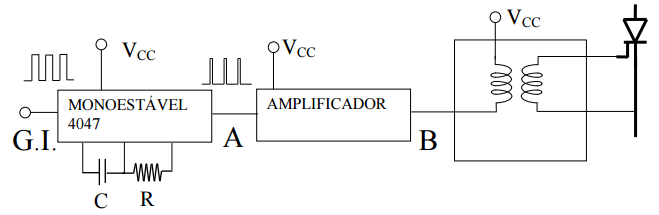
\includegraphics[width=\linewidth]{img/trigger_circuit}
	\caption{Circuito de Disparo}
	\label{fig:circuit_1}
\end{figure}

O objetivo neste trabalho é assim realizar este circuito com uma frequência de $1$ kHz fazendo para isso uso de um sinal com esta frequência originado por um Gerador de Impulsos (GI). O circuito de disparo será então composto por uma monoestável que reage ao flanco ascendente do sinal originado pelo GI; tem-se assim à saída da monoestável um impulso cuja duração será função da resistência R e condensador C. A duração deste impulso deve ser definida consoante as características da Gate do tirístor que se está a utilizar, sendo neste caso de $10$ $\mu$s. Este impulso tem no entanto que ser amplificado para que seja injetada corrente suficiente na Gate do tirístor. Usa-se assim um transístor de ganho elevado transitando da saturação ao corte, estabelecendo uma tensão no primário do transformador, sempre que surja o impulso na saída da monoestável. As formas de onda destes impulsos podem ser observadas na \autoref{fig:circuit_2}.

\begin{figure}[h]
	\centering
	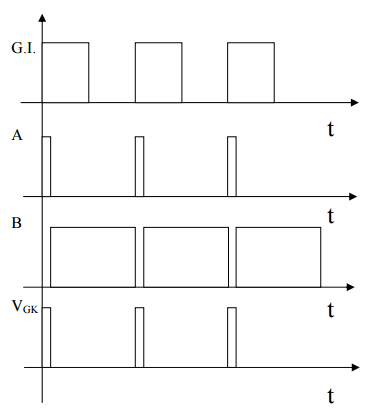
\includegraphics[width=\linewidth]{img/trigger_waveform}
	\caption{Formas de onda das tensões no circuito de disparo}
	\label{fig:circuit_2}
\end{figure}

O transformador serve também para que se obtenha o isolamento galvânico entre os circuitos de disparo e potência.

\section{Montagem e equipamento}

A montagem presente na placa impressa utilizada no laboratório pode ser observada na \autoref{fig:circuit_3}.

\begin{figure}[h]
	\centering
	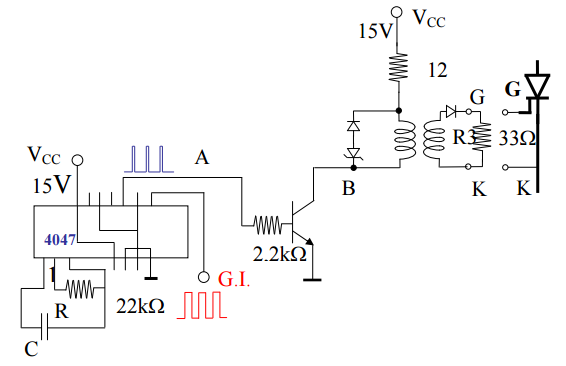
\includegraphics[width=\linewidth]{img/assembly_circuit}
	\caption{Esquema elétrico do circuito de disparo presente na placa impressa}
	\label{fig:circuit_3}
\end{figure}

Tal como dito na secção acima, a duração do impulso será definida por R e C segundo a seguinte fórmula dada pelo fabricante:

$$ T = 2.88 \, R \, C $$

Para que se tenha $10$ $\mu$s faz-se assim uso de uma resistência com $10$ k$\Omega$ e $0.4$ nF, sem necessidade de uma grande precisão nos valores pois a exatidão do tempo de disparo neste circuito não é prevalente.

O equipamento a utilizar na condução do trabalho é assim:

\begin{itemize}
\item 1 Osciloscópio;
\item 1 Sonda de corrente;
\item 1 Gerador de impulsos;
\item 2 Fontes de alimentação;
\item 2 Multímetros;
\item 1 Placa de circuito impresso;
\end{itemize}

\section{Condução do Trabalho}
\end{document}
